\documentclass[11pt,a4paper]{article}
\usepackage[utf8]{inputenc}
\usepackage[T1]{fontenc}
\usepackage{geometry}
\geometry{margin=2.5cm}
\usepackage{booktabs}
\usepackage{array}
\usepackage{xcolor}
\usepackage{listings}
\usepackage{hyperref}
\usepackage{float}
\usepackage{enumitem}

\lstdefinestyle{Cstyle}{
  language=C,
  basicstyle=\ttfamily\footnotesize,
  numbers=left,
  numberstyle=\tiny,
  frame=single,
  breaklines=true,
  tabsize=2,
  commentstyle=\color{gray},
  keywordstyle=\color{blue},
  stringstyle=\color{red},
}
\lstdefinestyle{asmstyle}{
  language={[x86masm]Assembler},
  basicstyle=\ttfamily\footnotesize,
  numbers=left,
  numberstyle=\tiny,
  frame=single,
  breaklines=true,
  tabsize=2,
  commentstyle=\color{gray},
}

\hypersetup{
  colorlinks=true,
  pdftitle={BradISA V2 Extensions},
  pdfauthor={Brad Devices},
}

\usepackage{bradbrand}

\begin{document}
\bradtitlepage{BradISA V2 Extensions}{%
  \textbf{BradISA V2 Extensions}}{%
  Compressed ISA, Vector, and Power Management Architecture}{%
  Revision 2.1 --- July 2026}
\newpage

\section{V2 Overview}

BradISA V2 extends V1 with four major additions:
\begin{enumerate}[nosep]
  \item \textbf{16-bit compressed instructions} --- two 16-bit instructions
        packed per 32-bit word, reducing code size by $\sim$30--40\%
  \item \textbf{New pipeline models} --- Kestrel (8-stage dual-issue in-order)
        and Falcon-Lite (3-stage ultra-tiny) to span the efficiency range
  \item \textbf{Vector extension (VSET)} --- 32 $\times$ 256-bit registers,
        integer/FP elementwise ops, memory ops, reductions, and converts
  \item \textbf{Power management subsystem} --- 24 MSRs, 5 power states,
        DVFS control, performance counters, clock-gating
\end{enumerate}

\newpage

\section{Compressed Instruction Format}

Compressed mode is activated by setting bit~4 (C) in the STATUS MSR.
When C=1, PC advances by 2~bytes (halfword) and each halfword encodes one
16-bit instruction. Two 16-bit instructions pack into a single 32-bit
aligned word.

\subsection{16-bit Encoding}

\begin{table}[H]
\centering
\caption{16-bit compressed instruction format}
\begin{tabular}{clll}
\toprule
Format & Bits [15:12] & Bits [11:8] & Bits [7:0] \\
\midrule
CRRR & opcode & rd & \{rs1[3:0], rs2[3:0]\} \\
CRI  & opcode & rd & \{rs1[3:0], imm4[3:0]\} \\
CBR  & opcode & rs1 & offset8[7:0] \\
CMV  & 0xC    & rd  & imm8[7:0] \\
CNOP & 0xD    & --- & --- \\
\bottomrule
\end{tabular}
\end{table}

\begin{figure}[H]
\centering
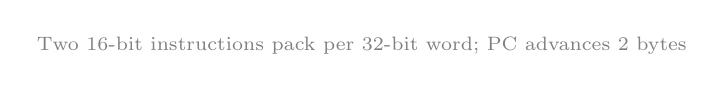
\begin{tikzpicture}[x=0.6cm]
  \bwfield{16}{CRRR --- 16-bit compressed}
  \bwslicen{12}{4}{op}
  \bwslicen{8}{4}{rd}
  \bwslicen{4}{8}{rs1}
  \bwslicen{0}{4}{rs2}
  \node[below, font=\scriptsize, gray] at (8,-1.1) {Two 16-bit instructions pack per 32-bit word; PC advances 2 bytes};
\end{tikzpicture}
\caption{CRRR format --- 16-bit compressed register-to-register encoding}
\end{figure}

\subsection{Compressed Opcode Map}

\begin{table}[H]
\centering
\caption{Compressed opcode mapping}
\begin{tabular}{cllc}
\toprule
Cop & Mnemonic & Format & Semantics \\
\midrule
0x0 & C.ADD  & CRRR & rd = rs1 + rs2 \\
0x1 & C.SUB  & CRRR & rd = rs1 - rs2 \\
0x2 & C.AND  & CRRR & rd = rs1 \& rs2 \\
0x3 & C.OR   & CRRR & rd = rs1 | rs2 \\
0x4 & C.XOR  & CRRR & rd = rs1 \^{} rs2 \\
0x5 & C.SHL  & CRRR & rd = rs1 $<<$ rs2[4:0] \\
0x6 & C.SHR  & CRRR & rd = rs1 $>>$ rs2[4:0] \\
0x7 & C.ADDI & CRI  & rd = rs1 + ZEXT(imm4) \\
0x8 & C.LDW  & CRI  & rd = mem[rs1 + ZEXT(imm4)$\times$4] \\
0x9 & C.STW  & CRI  & mem[rs1 + ZEXT(imm4)$\times$4] = rd \\
0xA & C.BZ   & CBR  & if (rs1==0) PC += SEXT(off8)$\times$4 \\
0xB & C.BNZ  & CBR  & if (rs1!=0) PC += SEXT(off8)$\times$4 \\
0xC & C.MV   & CMV  & rd = ZEXT(imm8) \\
0xD & C.NOP  & ---  & No operation \\
0xE & C.JMP  & CBR  & PC += SEXT(off8)$\times$4 \\
0xF & C.CALL & CBR  & LR = PC+2; PC += SEXT(off8)$\times$4 \\
\bottomrule
\end{tabular}
\end{table}

\subsection{Code Size Savings}
Compressed instructions reduce code size by $\sim$30--40\% compared to V1
fixed 32-bit encoding. Common instruction sequences (ADDI, MV, short
branches) benefit most. The assembler automatically packs two 16-bit
instructions per 32-bit word when {\tt .compress} mode is active.

\newpage

\section{Pipeline Models}

\subsection{Kestrel --- 8-stage Dual-Issue In-Order}

Kestrel is a mid-range core bridging the gap between Falcon (single-issue,
5-stage) and Phoenix (octa-issue OoO, 10-stage).

\begin{table}[H]
\centering
\caption{Kestrel pipeline characteristics}
\begin{tabular}{ll}
\toprule
Property & Value \\
\midrule
Pipeline depth & 8 stages \\
Issue width & Dual-issue \\
Execution & In-order \\
Branch predictor & Static BTFNT + 16-entry BTB \\
Load-to-use latency & 3 cycles (1 stall) \\
ALU forwarding & Full (no ALU stall) \\
Typical IPC & 1.2 \\
Peak IPC & 1.8 \\
Target DMIPS/MHz & 3.0 \\
Target frequency & 3.5 GHz \\
Target TDP & 3.5 W \\
DMIPS/W & 3,000 \\
\bottomrule
\end{tabular}
\end{table}

\subsubsection*{Pipeline Stages}
\begin{enumerate}[nosep]
  \item \textbf{F1} --- Instruction address generation, BTB lookup
  \item \textbf{F2} --- Instruction cache read
  \item \textbf{D1} --- Decode instruction~0, register file read
  \item \textbf{D2} --- Decode instruction~1, pairing check
  \item \textbf{EX1} --- ALU~0 / address generation
  \item \textbf{EX2} --- ALU~1 / data memory access
  \item \textbf{M} --- Memory result ready
  \item \textbf{WB} --- Writeback to register file
\end{enumerate}

\subsection{Falcon-Lite --- 3-stage Ultra-Tiny Core}

Falcon-Lite is designed for extreme low-power IoT and embedded
applications, targeting ${<}$500 LUTs on FPGA.

\begin{table}[H]
\centering
\caption{Falcon-Lite pipeline characteristics}
\begin{tabular}{ll}
\toprule
Property & Value \\
\midrule
Pipeline depth & 3 stages \\
Issue width & Single-issue \\
Execution & In-order \\
Register file & 8 $\times$ 32-bit (r0--r7) \\
Hardware MUL & No (returns 0) \\
Typical IPC & 0.55 \\
Peak IPC & 0.70 \\
Target DMIPS/MHz & 1.2 \\
Target frequency & 1.2 GHz \\
Target TDP & 0.16 W \\
DMIPS/W & 8,800 \\
FPGA LUTs & ${<}$500 \\
\bottomrule
\end{tabular}
\end{table}

\subsubsection*{Pipeline Stages}
\begin{enumerate}[nosep]
  \item \textbf{F} --- Fetch instruction, PC increment
  \item \textbf{D} --- Decode, register file read
  \item \textbf{EX} --- Execute, memory access, writeback
\end{enumerate}

\subsection{Efficiency Comparison}

\begin{table}[H]
\centering
\caption{All BradCore pipeline models}
\begin{tabular}{lcccc}
\toprule
Core & Stages & Issue & DMIPS/MHz & DMIPS/W \\
\midrule
Falcon-Lite & 3 & 1-wide & 1.2 & 8,800 \\
Falcon & 5 & 1-wide & 2.2 & 10,560 \\
Kestrel & 8 & 2-wide & 3.0 & 3,000 \\
Phoenix C & 10 & 8-wide OoO & 5.5 & 4,714 \\
Phoenix W & 10 & 8-wide OoO & 5.5 & 2,200 \\
\bottomrule
\end{tabular}
\end{table}

\newpage

\section{Vector Extension (VSET)}

BradISA V2 adds a 256-bit vector extension (VSET) that closes the SIMD gap
with ARM NEON/SVE2, RISC-V Vector~1.0, and Apple AMX for ML/AI, DSP, and
media workloads. VSET is the \textbf{only} floating-point facility in
BradISA V1/V2 --- scalar FP registers are not defined; FP scalars live in
vector register lane~0 and reductions deliver results through the vector
register file. VSET is the fixed-width (AVX-class) standard; the SVE-style
variable-length SVEXT path is scoped below as a Gen2 design intent, not a
shipped feature.

\subsection{Architecture Overview}

\begin{table}[H]
\centering
\caption{VSET architectural parameters}
\begin{tabular}{ll}
\toprule
Parameter & Value \\
\midrule
Vector registers & 32 ({\tt v0}--{\tt v31}), 256-bit each \\
Vector length (VLEN) & 256 bits (fixed) \\
Element widths (SEW) & 8, 16, 32, 64 bits \\
Elements per register & 32$\times$8-bit / 16$\times$16-bit / 8$\times$32-bit / 4$\times$64-bit \\
FP formats & FP32, FP64 (Gen1); FP16 (Gen2) \\
Mask register & {\tt v0} (reserved for Gen2 predication) \\
Primary opcode & {\tt 0xF} (VEXT group; {\tt 0xF0000000} remains {\tt RET}) \\
Vector unit enable & MSR~23 (VSTATUS.VE) \\
Issue rate & 1 vector op/cycle (Phoenix), 256-bit datapath \\
\bottomrule
\end{tabular}
\end{table}

VSET uses fixed-length 256-bit registers (rather than RISC-V's software-
tunable VLEN) so the vector datapath maps 1:1 onto a 256-bit SIMD lane ---
the same width as the BradVector GPU cores. A vector register therefore holds
8$\times$FP32, 4$\times$FP64, 8$\times$int32, 16$\times$int16, or
32$\times$int8.

\begin{figure}[H]
\centering
\begin{tikzpicture}[cell/.style={draw=bradgraylight, fill=bradgraylight!35}, esew/.style={draw=bradgolddark, fill=bradgolddark!30}, eseb/.style={draw=bradgolddark, fill=bradgolddark!20}]
  \foreach \i in {0,...,31}{ \draw[cell] (\i*0.42,0) rectangle (\i*0.42+0.42,0.55); }
  \foreach \i in {0,4,8,12,16,20,24,28}{ \draw[esew, line width=0.8pt] (\i*0.42,0) rectangle (\i*0.42+1.68,0.55); }
  \node[above, font=\scriptsize, text=bradgolddark] at (6.72,-0.1) {SEW=32 (FP32/int32): 8 lanes};
  \foreach \i in {0,...,15}{ \draw[eseb] (\i*0.84,0.9) rectangle (\i*0.84+0.84,1.45); }
  \node[above, font=\scriptsize, text=bradgolddark] at (6.72,0.8) {SEW=16 (FP16/int16): 16 lanes};
  \foreach \i in {0,...,31}{ \draw[esew] (\i*0.42,1.8) rectangle (\i*0.42+0.42,2.35); }
  \node[above, font=\scriptsize, text=bradgolddark] at (6.72,1.7) {SEW=8 (int8): 32 lanes};
  \node[below, font=\tiny, gray] at (6.72,-0.55) {bit 0 $\rightarrow$ bit 256 (8 bits/cell)};
\end{tikzpicture}
\caption{VSET 256-bit register lane layout --- SEW selects the active row; all lanes operate in lockstep}
\end{figure}


\subsection{Register File and ABI}

\begin{table}[H]
\centering
\caption{Vector register ABI conventions}
\begin{tabular}{cll}
\toprule
Register & ABI Name & Purpose \\
\midrule
{\tt v0}   & {\tt vm} & Mask register (Gen2 predication); zero-vector convention \\
{\tt v1}   & {\tt va0} & Vector argument~\#0 / return value \\
{\tt v2}   & {\tt va1} & Vector argument~\#1 \\
{\tt v3}   & {\tt va2} & Vector argument~\#2 \\
{\tt v4}   & {\tt va3} & Vector argument~\#3 \\
{\tt v5}--{\tt v7} & {\tt vt0}--{\tt vt2} & Caller-saved temporaries \\
{\tt v8}--{\tt v15} & {\tt vs0}--{\tt vs7} & Callee-saved \\
{\tt v16}--{\tt v31} & {\tt vt3}--{\tt vt18} & Caller-saved temporaries \\
\bottomrule
\end{tabular}
\end{table}

Callee-saved vector registers {\tt v8}--{\tt v15} must be preserved across
calls, matching the scalar callee-saved set {\tt r8}--{\tt r12}. The vector
calling convention passes the first four vectors in {\tt v1}--{\tt v4}; FP
scalars are passed in lane~0 of {\tt v1}--{\tt v4}.

\subsection{Encoding}

Vector instructions are 32-bit words with primary opcode {\tt 0xF}. The
fixed encoding {\tt 0xF0000000} remains the V1 {\tt RET} instruction for
backward compatibility; \textbf{all other} {\tt 0xF} encodings are vector
instructions. A 3-bit class field in bits [27:25] selects the functional
group.

\begin{table}[H]
\centering
\caption{Vector instruction formats}
\footnotesize
\begin{tabular}{clp{10cm}}
\toprule
Format & Class & Field layout (32-bit word) \\
\midrule
{\tt VV} & 000,001,011,100 & {\tt F} $\mid$ {\tt cls[27:25]} $\mid$ {\tt vd[24:20]} $\mid$ {\tt vs1[19:15]} $\mid$ {\tt vs2[14:10]} $\mid$ {\tt sew[9:8]} $\mid$ {\tt funct[7:0]} \\
{\tt VM} & 010 & {\tt F} $\mid$ {\tt cls[27:25]} $\mid$ {\tt vd[24:20]} $\mid$ {\tt base[19:16]} $\mid$ {\tt mop[15:13]} $\mid$ {\tt sew[12:11]} $\mid$ {\tt imm[10:0]} \\
{\tt VX} & 101 & {\tt F} $\mid$ {\tt cls[27:25]} $\mid$ {\tt vd[24:20]} $\mid$ {\tt vs1[19:15]} $\mid$ {\tt rs[14:11]} $\mid$ {\tt sew[10:9]} $\mid$ {\tt funct[8:0]} \\
{\tt VSC} & 110 & {\tt F} $\mid$ {\tt cls[27:25]} $\mid$ {\tt rd[24:21]} $\mid$ {\tt vs1[20:16]} $\mid$ {\tt resv[15:0]} \\
\bottomrule
\end{tabular}
\end{table}

{\tt F} = primary opcode {\tt 0xF} (bits [31:28]). {\tt sew}: 00=8-bit,
01=16-bit, 10=32-bit, 11=64-bit. {\tt vd}, {\tt vs1}, {\tt vs2} select
vector registers (5-bit); {\tt base}, {\tt rs}, {\tt rd} select scalar GPRs
(4-bit). No vector instruction may encode {\tt 0xF0000000}; such a word is
always {\tt RET}.

\begin{figure}[H]
\centering
\begin{tikzpicture}[x=0.48cm]
  \bwfield{32}{VV --- vector elementwise}
  \bwslicen{28}{4}{F}
  \bwslicen{25}{3}{cls}
  \bwslicen{20}{5}{vd}
  \bwslicen{15}{5}{vs1}
  \bwslicen{10}{5}{vs2}
  \bwslicen{8}{2}{sew}
  \bwslicen{0}{8}{funct}
\end{tikzpicture}
\caption{VV format --- vector elementwise encoding (F = primary opcode {\tt 0xF})}
\end{figure}

\subsection{Instruction Set}

\subsubsection*{VALU --- integer elementwise (class 000, VV)}

\begin{table}[H]
\centering
\caption{VALU operations}
\begin{tabular}{cllc}
\toprule
{\tt funct} & Mnemonic & Operands & Semantics \\
\midrule
0x01 & {\tt V.ADD}  & vd, vs1, vs2 & vd = vs1 + vs2 (element, wraps) \\
0x02 & {\tt V.SUB}  & vd, vs1, vs2 & vd = vs1 - vs2 \\
0x03 & {\tt V.MUL}  & vd, vs1, vs2 & vd = vs1 $\times$ vs2 (low bits) \\
0x04 & {\tt V.AND}  & vd, vs1, vs2 & vd = vs1 \& vs2 \\
0x05 & {\tt V.OR}   & vd, vs1, vs2 & vd = vs1 $|$ vs2 \\
0x06 & {\tt V.XOR}  & vd, vs1, vs2 & vd = vs1 \^{} vs2 \\
0x07 & {\tt V.SHL}  & vd, vs1, vs2 & vd = vs1 $<<$ vs2[$\log_2$(sew)$-$1:0] \\
0x08 & {\tt V.SHR}  & vd, vs1, vs2 & vd = vs1 $>>$ vs2[$\log_2$(sew)$-$1:0] (logical) \\
0x09 & {\tt V.MIN}  & vd, vs1, vs2 & vd = min(vs1, vs2) (signed) \\
0x0A & {\tt V.MAX}  & vd, vs1, vs2 & vd = max(vs1, vs2) (signed) \\
0x0B & {\tt V.CMPEQ} & vd, vs1, vs2 & vd = (vs1 == vs2) per element (all-ones / 0) \\
0x0C & {\tt V.CMPLT} & vd, vs1, vs2 & vd = (vs1 $<$ vs2) per element (signed) \\
0x0D & {\tt V.ABS}  & vd, vs1, --- & vd = $|$vs1$|$ per element (signed) \\
0x0E & {\tt V.MOV}  & vd, vs1, --- & vd = vs1 \\
\bottomrule
\end{tabular}
\end{table}

\subsubsection*{VFP --- floating-point elementwise (class 001, VV)}

\begin{table}[H]
\centering
\caption{VFP operations (SEW=32/64; IEEE-754-2019)}
\begin{tabular}{cllc}
\toprule
{\tt funct} & Mnemonic & Operands & Semantics \\
\midrule
0x01 & {\tt V.FADD}  & vd, vs1, vs2 & vd = vs1 + vs2 \\
0x02 & {\tt V.FSUB}  & vd, vs1, vs2 & vd = vs1 - vs2 \\
0x03 & {\tt V.FMUL}  & vd, vs1, vs2 & vd = vs1 $\times$ vs2 \\
0x04 & {\tt V.FMADD} & vd, vs1, vs2 & vd = vs1 $\times$ vs2 + vd (single rounding) \\
0x05 & {\tt V.FMIN}  & vd, vs1, vs2 & vd = fmin(vs1, vs2) \\
0x06 & {\tt V.FMAX}  & vd, vs1, vs2 & vd = fmax(vs1, vs2) \\
0x07 & {\tt V.FCMPEQ} & vd, vs1, vs2 & vd = (vs1 == vs2) per element \\
0x08 & {\tt V.FCMPLT} & vd, vs1, vs2 & vd = (vs1 $<$ vs2) per element \\
0x09 & {\tt V.FABS}  & vd, vs1, --- & vd = $|$vs1$|$ per element \\
0x0A & {\tt V.FNEG}  & vd, vs1, --- & vd = -vs1 per element \\
0x0B & {\tt V.FSQRT} & vd, vs1, --- & vd = $\sqrt{\mathrm{vs1}}$ per element \\
\bottomrule
\end{tabular}
\end{table}

FP16 (SEW=16) is a Gen2 option; Gen1 cores treat SEW=8/16 in VFP as an
undefined instruction.

\subsubsection*{VMEM --- vector memory (class 010, VM)}

\begin{table}[H]
\centering
\caption{VMEM operations}
\begin{tabular}{clll}
\toprule
{\tt mop} & Mnemonic & Semantics \\
\midrule
000 & {\tt V.LW} & vd[i] = mem[base + sext(imm11) + i$\times$(sew/8)] \\
001 & {\tt V.SW} & mem[base + sext(imm11) + i$\times$(sew/8)] = vs2[i] \\
010 & {\tt V.LWG} & Gather (Gen2) --- reserved \\
011 & {\tt V.SWG} & Scatter (Gen2) --- reserved \\
\bottomrule
\end{tabular}
\end{table}

Number of elements transferred per instruction is {\tt VLEN/sew}. {\tt V.LW}
uses {\tt vs2} as the destination in the {\tt VM} layout ({\tt vd} field);
{\tt V.SW} uses {\tt vd} as the store-data vector. The effective base address
{\tt base + sext(imm11)} must be aligned to {\tt sew/8} bytes; a misaligned
access raises the unaligned-access exception.

\subsubsection*{VRED --- reductions (class 011, VV)}

Reductions read the full source vectors and place the single result in lane~0
of {\tt vd}; all other lanes are zeroed. FP reductions accumulate in the
selected FP precision with single rounding at the end.

\begin{table}[H]
\centering
\caption{VRED operations}
\begin{tabular}{cllc}
\toprule
{\tt funct} & Mnemonic & Operands & Semantics \\
\midrule
0x01 & {\tt V.SUM}  & vd, vs1, --- & vd[0] = $\Sigma$ vs1 (integer, SEW) \\
0x02 & {\tt V.FSUM} & vd, vs1, --- & vd[0] = $\Sigma$ vs1 (FP32/FP64) \\
0x03 & {\tt V.MAX}  & vd, vs1, --- & vd[0] = max(vs1) (signed) \\
0x04 & {\tt V.MIN}  & vd, vs1, --- & vd[0] = min(vs1) (signed) \\
0x05 & {\tt V.FMAX} & vd, vs1, --- & vd[0] = fmax(vs1) \\
0x06 & {\tt V.FMIN} & vd, vs1, --- & vd[0] = fmin(vs1) \\
0x07 & {\tt V.DOT}  & vd, vs1, vs2 & vd[0] = $\Sigma$ vs1[i] $\times$ vs2[i] (int, accumulate 2$\times$SEW) \\
0x08 & {\tt V.FDOT} & vd, vs1, vs2 & vd[0] = $\Sigma$ vs1[i] $\times$ vs2[i] (FP, single rounding) \\
\bottomrule
\end{tabular}
\end{table}

{\tt V.DOT} is the int8 ML workhorse: at SEW=8 it computes a 32-lane
dot product into a 32-bit result in one instruction.

\subsubsection*{VCVT --- convert (class 100, VV)}

\begin{table}[H]
\centering
\caption{VCVT operations}
\begin{tabular}{cllc}
\toprule
{\tt funct} & Mnemonic & Operands & Semantics \\
\midrule
0x01 & {\tt V.CVT.SF} & vd, vs1, --- & signed int $\rightarrow$ FP (round-to-nearest) \\
0x02 & {\tt V.CVT.FS} & vd, vs1, --- & FP $\rightarrow$ signed int (round toward zero) \\
0x03 & {\tt V.CVT.UF} & vd, vs1, --- & unsigned int $\rightarrow$ FP \\
0x04 & {\tt V.CVT.FU} & vd, vs1, --- & FP $\rightarrow$ unsigned int \\
0x05 & {\tt V.WIDEN}  & vd, vs1, --- & vd:vd+1 = widen(vs1); {\tt vd} even \\
0x06 & {\tt V.NARROW} & vd, vs1, --- & vd[127:0] = narrow(vs1) \\
\bottomrule
\end{tabular}
\end{table}

{\tt V.WIDEN} doubles the element width (SEW $\rightarrow$ 2$\times$SEW) across a
register pair: {\tt vd} holds elements [0, N/2$-$1], {\tt vd+1} holds
[N/2, N$-$1]. {\tt vd} must be even. {\tt V.NARROW} halves the element width;
the result occupies the low 128 bits of {\tt vd}.

\subsubsection*{VSPL --- scalar-vector (class 101, VX)}

\begin{table}[H]
\centering
\caption{VSPL operations ({\tt rs} = scalar GPR)}
\begin{tabular}{cllc}
\toprule
{\tt funct} & Mnemonic & Operands & Semantics \\
\midrule
0x01 & {\tt V.BCAST} & vd, ---, rs & vd = broadcast(rs) to all lanes \\
0x02 & {\tt V.ADDX}  & vd, vs1, rs & vd = vs1 + rs \\
0x03 & {\tt V.SUBX}  & vd, vs1, rs & vd = vs1 - rs \\
0x04 & {\tt V.MULX}  & vd, vs1, rs & vd = vs1 $\times$ rs \\
0x05 & {\tt V.FADDX} & vd, vs1, rs & vd = vs1 + rs (FP) \\
0x06 & {\tt V.FMULX} & vd, vs1, rs & vd = vs1 $\times$ rs (FP) \\
0x07 & {\tt V.INS}   & vd, vs1, rs & vd = vs1 with lane~0 = rs \\
\bottomrule
\end{tabular}
\end{table}

For SEW $<$ 32, {\tt rs} is truncated to {\tt sew} bits before broadcast;
for SEW=64 it is sign-extended.

\subsubsection*{VSC --- scalar extract (class 110, VSC)}

\begin{table}[H]
\centering
\caption{VSC operation}
\begin{tabular}{cllc}
\toprule
{\tt funct} & Mnemonic & Operands & Semantics \\
\midrule
0x01 & {\tt V.EXT} & rd, vs1, --- & rd = vs1 lane~0 (zero/sign-extended to 32 bits) \\
\bottomrule
\end{tabular}
\end{table}

{\tt V.EXT} is the scalar read path that pairs with reductions and {\tt V.INS}.

\subsection{Vector Status MSR}

\begin{table}[H]
\centering
\caption{MSR 23 --- VSTATUS}
\begin{tabular}{cll}
\toprule
Bit & Flag & Description \\
\midrule
0   & VE    & Vector unit enable. 0 $\Rightarrow$ any vector instruction traps \\
    &       & (undefined instruction, cause 1) \\
1--4 & resv & Reserved \\
5   & VILL  & Sticky: illegal vector encoding executed \\
6   & VFP   & Sticky: FP exception flag (NaN produced, overflow) \\
\bottomrule
\end{tabular}
\end{table}

{\tt VILL} and {\tt VFP} are sticky flags written by the hardware and cleared
only by software (write 1 to clear). Gen1 FP never traps; NaN is propagated
per IEEE-754-2019 and {\tt VFP} is set.

\subsection{Example --- SAXPY}

The classic single-precision {\tt y[i] = a*x[i] + y[i]} loop, 8 elements per
vector operation:

\begin{lstlisting}[style=asmstyle]
    ; r1=x, r2=y, r3=n, r4=&a (8xFP32 per register)
saxpy:
    V.BCAST v2,  --, r4      ; v2 = a broadcast
    V.LW    v3,  r1, 0       ; v3 = x[0..7]
    V.FMUL  v3,  v3, v2      ; v3 = a * x
    V.LW    v4,  r2, 0       ; v4 = y[0..7]
    V.FADD  v3,  v3, v4      ; v3 = a*x + y
    V.SW    r2,  v3, 0       ; y[0..7] = v3
    ADDI    r1, r1, 32       ; advance 8 floats
    ADDI    r2, r2, 32
    ADDI    r3, r3, -8
    BNZ     r3, saxpy
    RET
\end{lstlisting}

\subsection{Autovectorization Notes}

\begin{itemize}[nosep]
  \item Clang/LLVM target hooks map {\tt <8 x float>}, {\tt <4 x double>},
        {\tt <8 x i32>}, {\tt <16 x i16>}, {\tt <32 x i8>} vectors directly
        onto one register --- no lane splitting or permutation code needed.
  \item Tail handling uses the scalar core: remaining elements use the
        {\tt r}-register ALU after the {\tt V.*} loop finishes.
  \item {\tt V.FMADD} and {\tt V.FDOT} preserve the LLVM
        {\tt contract} fast-math contract, enabling fused multiply-add codegen.
  \item int8 ML kernels map {\tt V.DOT} from LLVM reduction
        intrinsics and {\tt @llvm.fmuladd} on {\tt <32 x i8>}.
  \item {\tt VSTATUS.VE} is set once by the OS at context switch; the vector
        register file is part of the architectural state and saved/restored
        by the kernel, preserving {\tt v8}--{\tt v15} per ABI.
\end{itemize}

\subsection{Scopeable Vector Extension (SVEXT) --- [Gen2 Planning]}

On the question of AVX vs.\ SVE equivalents: VSET is the \textbf{AVX
counterpart} --- a fixed 256-bit SIMD standard with one datapath width and
stable code generation. That is deliberate and stays.

SVE-style \emph{variable-length} vector support (SVEXT) is \textbf{planned
for the Gen2 window}, not shipped now, for three honest reasons:
scalar/VSET code covers today's shipping software; a variable-length VLA
model changes the ABI and toolchain in ways the Gen1 compiler/OS stack is
not ready for; and the chip area is better spent on the BradVector GPU
engines that already absorb wide-SIMT workloads. SVEXT is therefore a
\emph{design intent}, explicitly not yet a committed feature, so no spec
is fabricated here. Intended Gen2 shape (subject to change):

\begin{itemize}[nosep]
  \item VLEN 128--512\,bit, variable length per processor (SVE-style
        vector-length agnostic code, {\tt PTRUE}/\texttt{WHILELT}-class
        vector-length predication).
  \item Same {\tt v0} register file uplifted to dynamic lengths, keeping
        the VSET ABI as the portable baseline and letting SVL be probed
        via a new {\tt VSTATUS.SVL} field or an {\tt ID\_VECTOR} MSR.
  \item Narrow (video/DSP) code stays on fixed VSET; HPC/AI loops compile
        to SVEXT where the VLEN pays for itself.
\end{itemize}

\newpage

\section{Power Management Subsystem}

\subsection{New MSRs}

BradISA V2 adds 17 new MSRs --- 16 for power management and performance
monitoring plus MSR~23 (VSTATUS) for the vector extension:

\begin{table}[H]
\centering
\caption{V2 MSR additions}
\begin{tabular}{cll}
\toprule
Index & Mnemonic & Description \\
\midrule
8  & PM\_CTRL   & Power management control \\
9  & PSTATE     & Current P-state \\
10 & PSTATES    & Available P-states bitmap \\
11 & VOLTAGE    & Core voltage in mV \\
12 & FREQ       & Core frequency in MHz \\
13 & ENERGY     & Accumulated energy in $\mu$J \\
14 & PWR\_CAP   & Power cap in mW \\
15 & TEMP       & Die temperature in $^\circ$C \\
16 & PERF\_CNT0 & Performance counter 0 \\
17 & PERF\_CNT1 & Performance counter 1 \\
18 & PERF\_CNT\_CTRL & Perf counter control \\
19 & L2\_PART   & L2 cache partitioning \\
20 & L3\_PART   & L3 cache partitioning \\
21 & CG\_MASK   & Clock-gating unit mask \\
22 & DBG\_CTRL  & Debug control \\
23 & VSTATUS   & Vector unit status (VE, VILL, VFP) \\
\bottomrule
\end{tabular}
\end{table}

\subsection{Power States}

The PM\_CTRL register encodes the current C-state in bits [3:0]:

\begin{table}[H]
\centering
\caption{Power C-states}
\begin{tabular}{ccll}
\toprule
State & Code & Name & Behaviour \\
\midrule
C0  & 0 & Active & Full operation \\
C1  & 1 & WFI & Clock-gated, instant wake \\
C1E & 2 & WFI + Vmin & Voltage reduced by 20\% \\
C2  & 3 & Sleep & Power-gated, cache retained \\
C2E & 4 & Sleep+ & Power-gated, cache flushed \\
C3  & 5 & Deep sleep & Full power-down, wake from IRQ \\
\bottomrule
\end{tabular}
\end{table}

\subsection{Status Register V2 Flags}

\begin{table}[H]
\centering
\caption{New STATUS register bits}
\begin{tabular}{cll}
\toprule
Bit & Flag & Description \\
\midrule
4 & C & Compressed mode enable \\
5 & EE & Energy-efficient mode hint \\
6 & DBG & Debug mode \\
\bottomrule
\end{tabular}
\end{table}

\subsection{Performance Counters}

PERF\_CNT\_CTRL configures two 32-bit counters (PERF\_CNT0, PERF\_CNT1),
assigning one event type to each:

\begin{table}[H]
\centering
\caption{Performance event selectors}
\begin{tabular}{cl}
\toprule
Code & Event \\
\midrule
0 & CPU cycles \\
1 & Instructions retired \\
2 & Branches \\
3 & Branch mispredicts \\
4 & Load-use stalls \\
5 & L1 cache misses \\
6 & L2 cache misses \\
7 & L3 cache misses \\
8 & Stall cycles \\
9 & IPC \\
\bottomrule
\end{tabular}
\end{table}

\subsection{Clock-Gating Mask}

The CG\_MASK register (MSR~21) controls per-unit clock gating. Each bit
corresponds to a pipeline unit:

\begin{table}[H]
\centering
\caption{Clock-gating unit mask}
\begin{tabular}{cl}
\toprule
Bit & Unit \\
\midrule
0 & Fetch \\
1 & Decode \\
2 & Rename \\
3 & Dispatch \\
4 & Issue \\
5 & Execute \\
6 & Memory \\
7 & Writeback \\
\bottomrule
\end{tabular}
\end{table}

\newpage

\section{Branch Predictor (Phoenix Optimisation)}

Phoenix can be configured with a tournament branch predictor:

\begin{table}[H]
\centering
\caption{Branch predictor configuration}
\begin{tabular}{ll}
\toprule
Parameter & Value \\
\midrule
Default type & Tournament (gshare + bimodal) \\
BTB size & 256 entries \\
BTB associativity & 4-way \\
Global history bits & 12 \\
Alternative types & None, Static BTFNT, 2-bit saturating \\
\bottomrule
\end{tabular}
\end{table}

\subsection{Load-Forwarding}

Phoenix supports load-to-use forwarding when the load result is consumed
within 2 cycles of the load instruction, reducing the load-use penalty
from 3 cycles to 1.

\newpage

\section{Revision History}

\begin{tabular}{lll}
\toprule
Revision & Date & Changes \\
\midrule
1.0 & July 2026 & Initial BradISA V1 specification --- Kinetic Gen1 \\
2.0 & July 2026 & Added V2 compressed instructions, Kestrel pipeline, \\
    &           & Falcon-Lite pipeline, power management MSRs, \\
    &           & branch predictor spec, performance counters \\
2.1 & July 2026 & Added Vector Extension (VSET): 32$\times$256-bit registers, \\
    &           & integer/FP elementwise ops, memory ops, reductions, \\
    &           & converts, VSTATUS MSR 23 \\
2.2 & July 2026 & Clarified VSET as the fixed-width (AVX-class) standard; \\
    &           & scoped SVEXT (SVE-style variable-length) as a Gen2 \\
    &           & design intent, not a shipped feature \\
\bottomrule
\end{tabular}

\end{document}
